\documentclass[fr]{../../../eplsummary}
\usepackage{../../../eplunits}

\newcommand*\textfrac[2]{\frac{\text{#1}}{\text{#2}}}

\hypertitle[']{Introduction à la gestion financière et comptable}{8}{FSA}{1290}
{Rodolphe de Schaetzen}
{André Nsabimana}

\section*{Chapitre 1. Les principes comptables}

\section{Les principes de quantification ou de mesure}
\subsection{Le principe de monétarisation}
Toutes les transactions sont exprimées en unités monétaires. On exclut donc les éléments non monnayables.
L'immatériel n'est pas appréhendé par la comptabilité, or c'est une richesse non négligeable d'une entité. Par exemple la capacité d'une société à innover et créer.

\medskip
Ce principe suppose la stabilité de l'unité monétaire dans le temps. Or les monnaies ont des taux qui varient et la valeur nette des acquis peut varier dans le temps. Prenons pour exemple une société Européenne libellée en EUR qui a une activité aux US, les comptes doivent être gardés en EUR en prenant en compte le taux de change actuel. Ou prenons l'exemple d'un immeuble acquis il y a de nombreuses années. Sa valeur réelle actuelle risque d'être éloignée de sa valeur nette comptable.

\subsection{Le principe des coûts historiques}
En droit comptable belge, pour évaluer la valeur d'un élément, on retient son coût historique. C'est-à-dire son coût d'acquisition ou son coût de production.

\medskip
Un premier correctif est effectué à la fin de chaque exercice comptable (durée: +/- un an) pour une partie des biens qui seront amortis pour enregistrer la diminution de valeur qu'ils ont subis.

\medskip
Un deuxième correctif consiste en la possibilité de revaloriser certaines catégories d'actifs. (Sous certaines conditions)

\subsection{le principe de prudence}
Le principe de prudence consiste à prendre immédiatement en compte une diminution probable de la valeur d'un bien alors qu'on ne prend en compte l'augmentation de valeur que lorsqu'on réalise réellement l'augmentation (revente ou autre).

\medskip
Cela évite la surestimation de la valeur du patrimoine d'une entité, mais à l'inverse on risque de sous-estimer sa valeur.

\medskip
Le principe de prudence a pour objectif premier d'inspirer la confiance dans les comptes publiés par les entreprises.

\section{Les principes d'observation}
\subsection{Le principe de l'entité}
``Chaque société ou organisation non-marchande est considérée comme une entité distincte de ses propriétaires, membres ou partenaires économiques.''
\begin{itemize}
    \item Entreprise sous forme sociétaire: a généralement une personnalité juridique distincte des personnes physiques ou morales qui sont les propriétaires.
    \item Entreprise individuelle: le patrimoine se confond avec celui de son propriétaire, mais où la compta isole le patrimoine personnel et les résultats professionels.
    \item Organisation non marchande: pareil que pour les sociétés avec une personne morale.
\end{itemize}

\subsection{Le principe de découpage du temps}
Un exercice comptable est d'une durée de plus ou moins un an. Cela ne doit pas forcément commencer en Janvier comme l'année civile (ex. les clubs de sports qui se calquent à la saison sportive).

Cela a pour but de rattacher les faits comptables à un exercice comptable, mais ça ne correspond pas tout le temps aux opérations de l'entité.

Les effets des transactions sont comptabilisés au moment où ils se produisent et sont enregistrés dans la comptabilité et états financiers qui se rapportent aux exercices comptables.

\subsection{Le principe de continuité}
L'entreprise compte continuer son activité dans les années à venir. Il faut donc qu'il y ait suffisamment de fonds pour pouvoir continuer l'activité l'année suivante.

\section*{Chapitre 2. Représentation synthétique du patrimoine et de son évolution}
\section{Le bilan "Balance Sheet"}
\subsection{Notion}
Le bilan est une photographie instantanée du patrimoine monnayable de l'entité. Comme pour une photo il faut en prendre régulièrement pour éviter que les sujets de la photo ne changent avec le temps.

Il faut donc des états financiers récents.

\subsection{Le passif}
Le passif comprend l'ensemble des ressources qui sont mises à la disposition de l'entité à la date d'établissement du bilan. 
\begin{itemize}
    \item Les capitaux propres:
    \begin{itemize}
        \item Capital des actionnaires
        \item Bénéfices conservés
        \item Pertes
    \end{itemize}
    \item Les dettes auprès des:
    \begin{itemize}
        \item Banques
        \item Fournisseurs
    \end{itemize}
\end{itemize}

\subsection{l'actif}
Tout ce qui est utilisé ou tous les emplois de fonds qui ont été effectués.
\begin{itemize}
    \item Immobilisations (elles permettent d'exercer son activité et donc de faire du profit) :
    \begin{itemize}
        \item brevets
        \item bâtiments
        \item équipements
        \item parts de sociétés
        \item \dots
    \end{itemize}
    \item Créances :
    \begin{itemize}
        \item clients livrés (du bien ou du service) qui doivent encore payer
        \item promesse de subvention de l'état à une organisation non-marchande
    \end{itemize}sur des clients (ou sur les pouvoirs publics)
    \item Marchandises et produits en stock destinés à être vendus
    \item Les avoirs monétaires (en caisse ou sur compte en banque)
\end{itemize}

\begin{center}
 actif = capitaux propres + dettes
\end{center}

\subsection{Le tableau de bilan}
Tableau sous la forme de deux colonnes: l'actif et le passif.
\begin{center}
 actif = passif
\end{center}

\section{Le compte de résultats}
\subsection{Notion}
Le compte de résultats représente la traduction comptable de l'évolution des activités de l'entité. Il synthétise au cours de l'année (sans prendre en compte la date d'encaissement ou de paiement):
\begin{itemize}
    \item les charges: les éléments qui influencent négativement la valeur de l'entité
    \item les produits: les éléments qui influencent positivement la valeur de l'entité
\end{itemize}

\begin{center}
 résultat = produits $-$ charges
\end{center}

La comptabilité d'engagement: basée sur produits et charges.

\medskip
La comptabilité de caisse: basée sur les recettes et les dépenses.

\medskip
On ne crée pas de compre de résultat après chaque transaction. On les enregistre dans le livre-journal. 

\section*{Chapitre 3. La Méthode Comptable: le Principe de la Partie Double}

\section{La comptabilité à partie double appliquée aux éléments du bilan}
\subsection{Principe}

\begin{center}
 Actif = Passif
\end{center}

\begin{center}
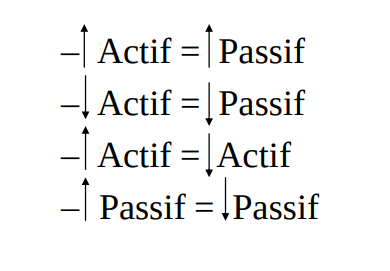
\includegraphics[scale = 0.3]{actif_passif.png}
\end{center}

\section{La comptabilité à partie double étendue aux éléments du résultat -  A FINIR}
Les enregistrements quotidiens combinent bilan et résultat, il serait donc simplificateur de ramener la comptabilité à des mouvements sur le bilan.

\subsection{Comptes de gestion}
Les comptes de gestion couvrent des emplois et des ressources définitifs pour une période donnée (exercice comptable).

Il existe 2 types de comptes de gestion:
\begin{itemize}
    \item Les comptes de charges: enregistrent les charges engagées ou subies par l'entité
\end{itemize}

\section*{Chapitre 4. L'Organisation du Traitement de l'Information Comptable}
\section{Le livre-journal}
Le livre-journal enregistre les transactions opération après opération. On comptabilise donc toutes les opérations en indiquant le compte du grand livre débité et le compte du grand livre crédité.
Au bas de chaque page du grand livre, il faut s'assurer de l'égalité des colonnes ``débit'' et ``crédit''.
Le livre-journal permet de retrouver la trace des opérations chronologiquement.
Il peut être divisé en journaux ``auxiliaires'' (par exemple journal des achats, journal des ventes, \dots )

\section{Le grand-livre}
Le grand-livre regroupe l'ensemble des comptes de l'entité. Il s'agit d'un résumé des transactions par compte. Cela permet de classer et récapituler les opérations.

\section{La balance des comptes}
Les soldes (débiteur ou créditeur), à une date
déterminé (fin de l’exercice comptable), des
comptes du grand-livre.

\section{Le livre d'inventaire}
\begin{itemize}
    \item L'inventaire
    \item Les règles d’évaluation: conversion des éléments à inventorier en unités monétaires 
    \item Le bilan, le compte de résultats et les annexes
\end{itemize}
\section{Methodologie du traitement comptable d'une opération}

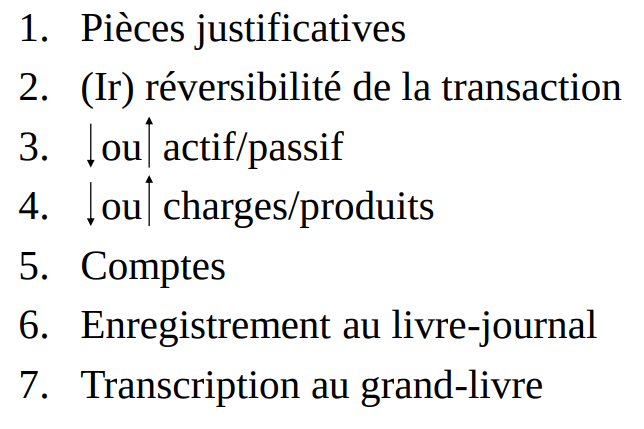
\includegraphics[scale = 0.25]{traitementcomptable.png}
\section*{Chapitre 6. Les Rubriques du Bilan}
\section{Les rubriques de bilan}
\subsection{Introduction aux rubriques de bilan}
Le bilan reflète en langage codé la situation patrimoniale de l'entité à un moment précis. Il recense :
\begin{itemize}
    \item du passif: les sources ou moyens de financement nécessaires aux investissements et à l'exploitation de l'entité.
    \begin{itemize}
        \item par ordre croissant de liquité
    \end{itemize}
    \item de l'actif: les utilisations ou emplois effectués par l'entité dans ses investissements et son exploitation. 
    \begin{itemize}
        \item par ordre décroissant d'exigibilité
    \end{itemize}
\end{itemize}
La rédaction du bilan respecte un schéma officiel belge (en rubriques en utilisant les chiffres romains).

Les actifs sont présentés en valeurs nettes, c'est-à-dire après réduction des amortissements et réductions de valeur cummulés. Il y a donc une perte d'information compensée par des indications supplémentaires dans l'annexe. Contradiction entre emplois et ressources: les amortissements sont des ressources qui permettent à l'entité de financer des emplois. 

\subsection{Rubriques de Passif}
\subsubsection*{Trois grandes masses}
Le passif se subdivise en 3 grandes masses:
\begin{itemize}
    \item Les capitaux propres: doivent couvrir le risque de l'entité (peut être négatif)
    \item Les provision (et impôts différés): pas de moyens propres et pas de dettes (liés à une future décision incertaine)
    \item Les dettes: les montants que l'entité doit rembourser
\end{itemize}

\subsubsection*{Capital}
Le capital correspond au patrimoine affecté de manière intangible aux besoins d'une entreprise par ses actionnaires ou associés, au moment de sa constitution ou suite à une augmentation de capital.

Le capital minimum est de 61 500€ pour les SA et de 18 550€ pour les SPRL.

Pour une entreprise individuelle, le capital ne s'agit pas du résultat de l'accumulation de bénéfices antérieurs. Le capital correspond aux moyens propres affectés durablement par la personne physique à son activité professionnelle.
\subsubsection*{Primes d'émission}
Imaginons A et B qui lancent une société et investissent 500 000€ chacun. Ils recoivent chacun 500 actions de 1000€. Apres quelques années, C vient augmenter le capital avec 1 500 000€ et en prenant compte des résultats de la société (plus-values latentes (à venir) + bénéfices + \dots), les actions valent maintenant 3 000€. C reçoit donc 500 actions et détient donc $1/3$ de la société. La différence entre la valeur nominale (1 000€) des actions et la valeur réelle (3 000€) constitue une prime d'émission des actions nouvelles. 
\subsubsection*{Moyens d'autofinancement}
Les moyens d'autofinancement correspondent aux ressources propres de l'entité qui financent les actifs.

Leur utilisation revêt des formes diverses:
\begin{itemize}
    \item La réserve légale (130): montant cumulé des bénéfices réalisé par certaines société qui ne peuvent pas être distribués par le droit des sociétés.
    \begin{itemize}
        \item Décidé par l'assemblée générale
        \item Au moins 1/20 des bénéfices nets par an dans la réserve
        \item Prélèvement de 1/20 jusqu'à atteindre 1/10 du capital social
        \item Permet de renforcer le capital et d'accroitre la garantie aux tiers
    \end{itemize}
    \item Les réserves indisponibles (131): bénéfices réalisés et réservés pour des décisions spéciales (p.e.: rachat de propres actions (1310))
    \item Les réserves immunisées (132): plus-values réalisées sur immobilisés. 
    \item Les réserves disponibles (133): à utiliser dans le futur par une décision à la majorité
    \item Le bénéfice reporté (14): bénéfice ni distribué, ni reporté
    \item La perte reportée (14): pour ``nettoyer'' le bilan de pertes reportées: réduction de capital ou prélèvement sur la réserve légale ou les primes d'émission. 
\end{itemize}

\subsubsection*{Plus-values de réévaluation (12)}
Permet de comptabiliser l'augmentation de valeur d'un bien (p.e.: terrain)

Sous certaines conditions strictes (augmentation de la valeur doit être durable), on peut comptabiliser des plus-values latentes (non-réalisées).

le droit comptable belge tend à décourager/canaliser la réévaluation des actifs (principe de prudence). 

\subsubsection*{Subsides en capital (15)}
Subventions accordées par les pouvoirs publics pour le financement d'investissements en immobilisations.

A la fin de l'exercice comptable on exerce une imputation au crédit du compte de résultats (produits financiers).

\subsubsection*{Provisions pour risques et charges (160-165)}
Pour couvrir des pertes ou charges futures qui sont probables à la date de clôture mais indéterminées au niveau du montant. (p.e.: grosses réparations, amendes, retour de produits, \dots)

\subsubsection*{Impots différés (168)}
Résultats de l'exercice comptable $\neq$ la base imposable.

\subsubsection*{Subdivisions de dettes}
\begin{itemize}
    \item Les dettes à plus d'un an (17): la partie des dettes qu'on ne devra pas rembourser dans les douze prochains mois.
    \item Les dettes à plus d'un an échéant dans l'année (42): la partie des dettes à plus d'un an (17) qu'on doit rembourser dans les douze mois.
    \item Les dettes à un an ou plus (43-48): les dettes à rembourser dans les 12 prochains mois.
\end{itemize}
\subsection{Rubriques d'actif}
\subsubsection*{Deux grandes masses}
\begin{itemize}
    \item Les actifs immobilisés (investissments): pas réalisés en numéraire (infrastructure - immobilisations)
    \item Les actifs circulants: valeurs disponibles ou réalisables (stocks, créances et liquidités)
\end{itemize}
Par exemple: une vache viandeuse est un actif circulant car elle sera transformée en liquidité une fois vendue. La vache laitière, elle, est un actif immobilisé car elle est maintenue durablement et amortie comme investissement productif de lait.

\subsubsection*{Frais d'établissement (20)}
A ne pas confondre avec les frais de bâtiments.

\medskip
Ce sont les frais rattachés à la constitution, développement ou restructuration de l'entité. 

\subsubsection*{Immobilisations incorporelles (21)}
Il s'agit d'investissements en éléments immatériels, tels que des frais de recherche et développement (R \& D), des brevets, une clientèle, \dots
\begin{itemize}
    \item Le goodwill: différence entre le coût d'acquisition d'une entreprise et la valeur réelle actuelle de cette entreprise (son actif)
\end{itemize}

\subsubsection*{Immobilisations corporelles (22-27)}
Il s'agit d'investissements en éléments matériels tels que des terrains, des constructions, des installations, des machines, de l'outillage, du mobilier, du matériel roulant, \dots

Les biens détenus en location-financement (leasing) doivent être portés sous les immobilisations corporelles.

Les actifs corporels subissent des amortissements (pas pour des terrains):
\begin{center}
(Coût d’acquisition $-$ valeur résiduelle) / période d’utilisation économique
\end{center}

\subsubsection*{Immobilisations financières (28)}
Il s'agit d'investissements en titres et en créances, tels que des actions ou prêts à des filiales. Plus généralement dans des entreprises avec lesquelles un lien durable et spécifique est établi (en vue d'augmenter le nombre de commandes d'un client par exemple).
\subsubsection*{Subdivision des créances}
\begin{itemize}
    \item Créances à plus d'un an (29): plutôt des prêts
    \item Créances à un an ou plus (40-41): échéances dans les 12 mois. 
\end{itemize}
\subsubsection*{Stocks et commandes en cours d'exécution}
\begin{itemize}
    \item Approvisionnements (matières premières et fournitures)(coût d'acquisition) (30-31)
    \item Marchandises (coût d'acquisition) (34)
    \item Produits finis (coût de production/revient) (33)
    \item Commandes en cours d'exécution. Quelle est la valeur à la fin de l'exercice comptable? (32-37)
\end{itemize}
Il y a des règles d'évaluation spécifiques: LIFO, FIFO, CMP, \dots
\subsubsection*{Placements de trésorerie (50-53)}
Il s'agit des placements bancaires sur compte et en valeurs mobilières (actions, obligations, \dots) sans avoir de caractère d'immobilisations financières (donc sans lien durable et spécifique).

\subsubsection*{Valeurs disponibles (55-57)}
Il s'agit des comptes financiers à vue et caisse. 
Si le solde est négatif, ils figurent au passif (433).
\section*{Chapitre 7. Les Rubriques du Compte de Résultats}
\section{Rubriques du compte de résultats}
\subsection{Intruduction}
Le compte des résultats assure la traduction en langage comptable (codé) de l'évolution des activités de l'entité au cours d'une période donnée. Il synthétise les charges et les produits.

\medskip
Les rubriques du compte de résultats sont classées par ordre décroissant du lien qu'elle entretiennent avec l'activité habituelle de l'entité. 
\begin{itemize}
    \item Produits et charges d'exploitation (liés à l'activité habituelle)
    \item Produits et charges financiers (ex. intérêts)
    \item Produits et charges exceptionnels (ex. plus-values ou moins-values liées à la vente d'un actif immobilisé)
\end{itemize}
\subsection{Rubriques et sous-rubriques}
\begin{itemize}
    \item Le chiffre d'affaires (70): lié à l'activité habituelle (toujours hors TVA) (451 TVA à payer) sous déduction des réductions commerciales
    \item Approvisionnement et marchandises (60): lié au coût de revient direct des fabrications, sous déduction des réductions commerciales (HTVA -> 411 TVA à récupérer).
    \item Services et biens divers (61): lié à l'exploitation de l'entité (coûts indirects)
    \item Rémunérations (62)
    \item Amortissements, réductions de valeur et provisions pour risques et charges (63) 
    \item Autres charges d'exploitation (64)
    \item Charges financières (65) (ex. intérêts)
    \item Charges exceptionnelles (66) (ex. réductions de valeur exceptionnelles)
    \item Impôts (67)
\end{itemize}
\subsection{Affectation des résultats}
A la fin de l'exercice comptable il faut:
\begin{itemize}
    \item Rédiger le compte de résultats (calculer le résultat)
    \item Décider sur l'affectation du résultat (ex. créer des réserves, dividendes, reporter,\dots)
    \item Rediger le bilan en tenant compte de l'affectation du résultat
\end{itemize}
\section*{Chapitre 8. Comptabilité de quelques opérations particulières}
\section{Comptabilité de quelques opérations particulières}
\subsection{Les variations de stocks}
Les stocks forment souvent une composante essentielle de l'actif d'une entité.
Cela ne veut pas dire qu'il ne faut pas inclure la variation des stocks dans le compte des résultats.

En réalité:
\begin{itemize}
    \item On achète des marchandises (prix d'achat) et on les revend (prix de vente)
    \item On fabrique des produits et on les vend (coût de production $\iff$ prix de vente)
    \item A la fin de l'exercice comptable, les unités achetées ou fabriquées ne sont pas toutes déjà vendues.
\end{itemize}

\subsubsection*{La démarche comptable}
En cours d'exercice il faut comptabiliser les achats et les ventes.
En fin d'exercice, il faut intégrer les variations des stocks dans le résultat de \textbf{l'activité}. Dans le compte de résultat de \textbf{l'exercice}, on ne doit prendre en charge que le coût de production des unités \textbf{vendues}.
On a donc:

\medskip
Si 
\begin{center}
 nombre d’unités achetées/fabriquées > le nombre d’unités vendues,
\end{center}
alors le stock augmente car les unités achetées/fabriquées de cet exercice comptable ne sont pas toutes déjà vendues. Donc le coût de production (prix d’achat) des unités vendues est inférieur au coût de production (prix d’achat) des unités fabriquées/achetées. Ce dernier a été enregistré en cours d’exercice, donc on doit enregistrer une diminution des charges d’exploitation à la fin de l’exercice.

Si 
\begin{center}
 nombre d’unités achetées/fabriquées < le nombre d’unités vendues,
\end{center}
alors le stock diminue car on a dû prendre des unités fabriquées/achetées et stockées pendant l’exercice précédente. Donc le coût de production (prix d’achat) des unités vendues est supérieur au coût de production (prix d’achat) des unités fabriquées/achetées. On doit prendre en charge dans cet exercice une partie du coût de production (prix d’achat) des unités fabriquées/achetées à l’exercice précédent, donc on doit enregistrer une augmentation des charges d’exploitation à la fin de l’exercice.

\subsubsection*{Valeur des unités de stock}
Si les prix d'achat et le coût de production restent constants durant l'exercice: aucun problème.

Si les prix ou les coûts varient durant l'exercice. On a 3 manières de valoriser la consommation de stock:
\begin{itemize}
    \item FIFO (first in, first out): les premiers stocks seront les premiers vendus
    \item LIFO (last in, first out): les derniers stocks seront les premiers vendus
    \item PMP (prix moyen pondéré): on recalcule avant chaque sortie la valeur d'acquisition moyenne des éléments en stock
\end{itemize}
Le choix de la méthode de valorisation a un impact sur le résultat opérationnel de l'exercice! Dès qu'on a choisi une méthode de valorisation, on ne peut plus la changer. Voir exemple livre p.93.
\subsubsection*{Ecriture comptable}
\begin{itemize}
    \item Augmentation, diminution des stocks de marchandise, approvisionnement:
    \begin{itemize}
        \item Classe 3: 300, 310 ou 340
        \item Classe 6: 6094
    \end{itemize}
    \item Augmentation, diminution des stocks de produits finis
    \begin{itemize}
        \item Classe 3: 330
        \item Classe 7: 713
    \end{itemize}
    \item ?
\end{itemize}

\subsection{Les frais de personnel}
(section a retravailler)
\subsubsection*{Calcul des rémunérations et du coût salarial}
Sur le salaire brut, l'employeur retient d'abord les cotisations personnelles de sécurité sociale (\SI{13.07}{\percent}). Ensuite il retient le précompte professionnel. Le solde constitue la rémunération nette du travailleur.

\medskip
Par ailleurs l'employeur paie des cotisations patronales de sécurité sociale (jusqu'à environ \SI{35}{\percent} du salaire brut), l'assurance accident du travail, d'éventuelles assurances extra-légales, le coût de l'administratif, \dots
\subsubsection*{Personnel intérimaire, gérants, administrateurs}
Ils sont tous considérés comme des prestataires des services (617/618). Il n'y a donc pas de côtisation patronale de sécurité sociale à payer ainsi que pas de cotisation ONSS personnelle et précompte professionnel à précompter. 
 
\subsubsection*{Pécules de vacances et gratifications de fin d'année}
La pécule de vacances est basée sur les prestations de l'année précédente, donc à la fin de l'exercice comptable, on doit la considérer comme un coût salarial (623) et une dette latente aux employées (456)

On part du même principe pour les gratifications/primes de fin d'année (623/457)

\subsubsection*{Résumé}
\begin{center}
    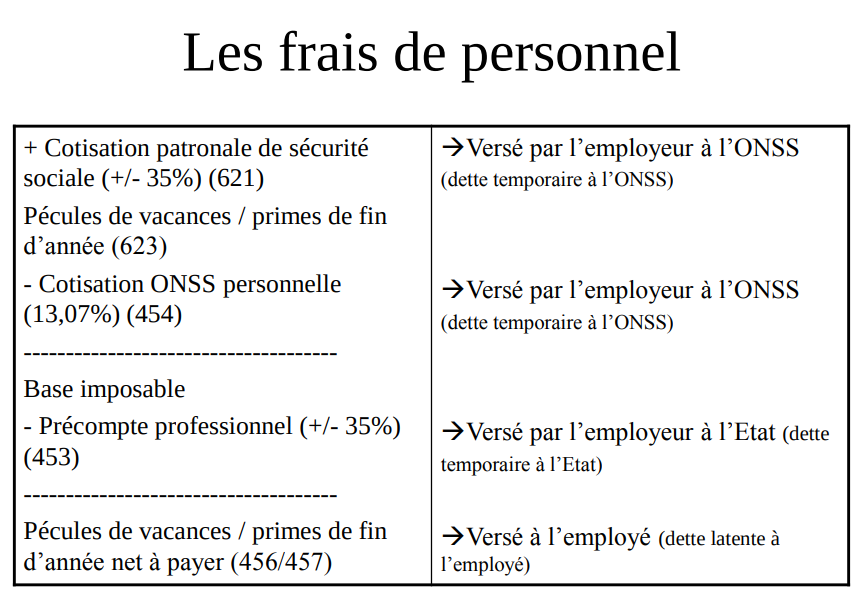
\includegraphics[scale=0.25]{frais_personnel.png}
\end{center}

\subsection{Les amortissements}
Les actifs immobilisés représentent l’infrastructure (la capacité de production) de l’entité qui n’est pas ``consommée'' immédiatement. L’usage de l’ infrastructure permet de générer des avantages économiques (créer de la valeur) pendant plusieurs années. C’est l’usage de l’infrastructure qui cause une perte de sa valeur.

L'amortissement doit refléter l'utilisation réelle d'un actif. Souvent les amortissements sont aussi inspirés par des considérations fiscales (= charge déductible).

\medskip
La non-utilisation d'un actif n'exclut pas son amortissement.
On amortit:
\begin{itemize}
    \item Les frais d'établissement
    \item Les immobilisations incorporelles
    \item Les immobilisations corporelles (sauf terrains)
\end{itemize}
Par contre, on n'ammortit \textbf{pas} les immobilisations financières.

\subsubsection*{Les méthodes d'amortissements}
\begin{itemize}
    \item L'amortissement linéaire: l'amortissement annuel reste le même pendant la durée de vie de l'actif, c'est la méthode la plus simple, mais elle ne reflète pas toujours la réalité économique. Utilisé pour des frais d'établissement, des immobilisations incorporelles, des bâtiments et des voitures.
    \item L'amortissement basé sur l'utilisation de l'actif: l'amortissement annuel correspond à l'utilisation réelle de la capacité pendant l'année. Eventuellement utilisé pour des installations, machines et outillage (pas évident d'estimer en avance la capacité réelle).
    \item L'amortissement dégressif:
    \begin{itemize}
        \item Egal au double du taux linéaire correspondant à une durée de dépréciation normale du bien (2x le taux linéaire)
        \item Base amortissable d'année en année: le solde non-encore amorti au terme de l'exercice précédent. Le taux doublé s'applique sur la valeur résiduelle
        \item Dotation annuelle maximale = \SI{40}{\percent} de la valeur d'acquisition.
        \item Retour à l'équivalent linéaire dès que la méthode linéaire aura livré une dotation plus importante
        \item Utilisé pour des installations, machines, outillage qui perdent la plupart de leur valeur dans les premières années d'usage
        \item Interdit pour des voitures ou immobilisations corporelles
    \end{itemize}
\end{itemize}
\subsubsection*{Amortissements et réductions de valeur}
Les amortissements et les réductions de valeur ont en commun qu'ils ont pour effet de convertir des débits figurant à l'actif en débits correspondant à des charges. Leurs écritures comptables sont assez voisines.

\medskip
Les amortissements sont annuels et pour des actifs dont l'utilisation est limitée dans le temps.

\medskip
Les réductions de valeurs sont occasionnels et pour des actifs dont l'utilisation n'est pas limitée dans le temps (ex. un terrain) et pour les autres éléments d'actifs (les stocks, les créances et les placements).
\subsubsection*{Ecriture comptable générique pour une réduction de valeur}
Augmentation des charges (631-634).
Diminution de la valeur des actifs amortis (3..9/409/419/5..9) -> compte correcteur d'actif

\subsection{Les provisions}
Principe des provisions: la ``décision'' est prise, mais le montant n'est pas encore défini/certain. Donc on est sûr de devoir payer, mais on ne sait pas exactement combien.
Une provision a pour but de surtout répartir le futur impact comptable d'une grande décision sur plusieurs années. Cela évite un résultat largement négatif dans un des exercices comptables suivants.

Une provision a également pour bur d'optimiser la situation fiscale car une provision est déductible.
Il y a les provisions pour prépensions (635/160), pour grosses réparations et entretien (162/636) et provisions pour litiges en cours (673/163).
\subsubsection*{Ecriture comptable générique pour les provisions}
Au moment de la constitution de la provision:
\begin{itemize}
    \item Augmentation des charges (635/636637)
    \item Augmentation du passif (160/162/123)
\end{itemize}
Au moment de la survenance effective de la charge:
\begin{itemize}
    \item Diminution du passif (160/162/123) -> utiliser la provision
    \item Diminution des charges (6351/6361/6371) -> neutraliser la charge effectivement subie
    \item Augmentation des charges effectives (61)
    \item Augmentation des dettes (440)
\end{itemize}
Une provision n'entraine aucune sortie d'argent. C'est une charge et non une dépense.

\section*{Chapitre 10. La demande d'information financière, ses sources et ses thèmes fondamentaux}
\section{L'analyse financière}
\subsection{Introduction}
L'analyse financière constitue un ensemble de concepts, de méthodes et d'instruments qui permettent de formuler une appréciation relative à la situation financière d'une entreprise, aux risques qui l'affectent, au niveau et à la qualité de ses performances. 
C'est un outil de support pour la prise de décision et le contrôle.

\medskip
Exemples:
\begin{enumerate}
    \item Une entreprise a besoin de ressources (capital propre et dettes)
    \item Les actionnaires ou les banques (fournisseurs de ressources) veulent d'abord analyser la situation financière de l'entreprise avant d'accorder des ressources
    \item Dès qu'ils ont accordé des ressources, ils veulent rester au courant de la performance financière de l'entreprise
\end{enumerate}
\subsection{La demande d'information financière}
L'analyse financière doit faciliter la prise de décision, le contrôle de la performance et le suivi des contrats ou d'accords.
L'analyse financière intéresse différents groupes de d'acteurs.

\subsubsection*{Le groupe des investisseurs}
On peut distinguer deux types d'investisseurs:
\begin{itemize}
    \item L'actionnaire de contrôle: détient une part significative du capital, ce qui lui permet d'exercer une influence sur le long terme en terme de pérénnité et rentabilité.
    \item L'actionnaire financier: détient des actions en vue d'optimiser ka rentabilité de son investissement à CT ou MT.
\end{itemize}

\subsubsection*{Le groupe de créanciers}
Le groupe de créanciers comprend les banques fournisseurs, l'administration fiscale, l'ONSS. La question qui les intéresse est la capacité de l'entreprise à faire face à ses obligations.

Dans un premier temps l'entreprise doit avoir suffisament de liquidités pour couvrir les paiements dus à CT (factures fournisseurs, cotisations ONSS, \dots).

Dans un second temps l'entreprise doit avoir la capacité de générer du cash flow (solvabilité) pour assurer les paiements dus et la rentabilité qui est un déterminant de la capacité 
à générer de la liquidité au long terme. 

\subsubsection*{Le groupe des membres du personnel}
Il s'agit des dirigeants et cadres qui ont besoin de l'information financière pour simuler l'impact de futures décisions et pour calculer les rémunérations variables.
Les employés et ouvriers peuvent aussi y trouver un intérêt (sécurité de l'emploi). 

\subsubsection*{Le groupe des analystes et conseillers financiers}
Y trouvent une utilité en fonction de leurs clients: rentabilité, liquidité, politique de dividende, \dots

\subsubsection*{Le groupe des entreprises ou personnes en relations d'affaires avec l'entité}
Il peut s'agir:
\begin{itemize}
    \item des clients et fournisseurs (analyse de la liquidité ou solvabilité)
    \item des concurrents (potentiel stratégique)
    \item des acteurs pour fusions et acquisition (valorisation de l'entité)
\end{itemize}

\subsubsection*{Le groupe des institutions publiques, des pouvoirs subsidiants et des bailleurs de fonds du non-marchand}
Il peut s'agir:
\begin{itemize}
    \item de l'état (détermination de l'impôt des sociétés)
    \item du tribunal de commerce (signaux d'alarme pour sociétés en difficultés financières)
    \item des pouvoirs subsidiants (allouer des subsides ou non)
\end{itemize}

\subsubsection*{Le grand publique}

\subsection{Les sources d'information}
\subsubsection*{Les états financiers}
\begin{itemize}
    \item Le bilan: sitation du patrimoine à la date de cloture de l'exercice. 
    \item Le compte de résultats: synthèse de la gestion pour l'ensemble de l'exercice comptable
    \item Les annexes: informations supplémentaire qui commentent le bilan et le compte de résultats (ex. méthodes d'évaluations, \dots)
    \item Le bilan social: renseignements en matière d'effectifs, important dans les secteurs ou les frais de personnel représentent une part importante de la valeur ajoutée
\end{itemize}

\subsubsection*{Le rapport de gestion}
Destiné à l'assemblée générale. Comprend un commentaire sur la situation actuelle de l'entreprise, son évolution dans le temps et ces principaux risques et incertitudes. Comprend également les évènements survenus après la date de clôture ainsi que les plans stratégiques à court et long terme et les opérations affectant le capital de l'entreprise. 

\subsubsection*{Rapport du commissaire ou rapport de contrôle}
Entreprises qui sont obligées d'avoir un commisaire:
\begin{itemize}
    \item nombre effectifs > 100 employés temps plein (ETP)
    ou dépasse au moins 2 des seuils suivants
    \item nombre effectifs > 50 ETP
    \item CA (chiffre d'affaire annuel) > 7.3 millions d'euros
    \item total d'actif > 3.65 millions d'euros
\end{itemize}
Le réviseur d'entreprise contrôle:
\begin{itemize}
    \item la conformité au droit comptable. (Belge, Américain, IAS/IFRS, \dots)
    \item l'image fidèle au patrimoine, de la sitation financière et des résultats reflétées par les comptes annuels
    \item la conformité du rapport de gestion
    \item la conformité aux statut et dispositions légales
\end{itemize}

\subsubsection*{Les comptes consolidés}
Utile pour les groupes d'entreprises. Une entreprise qui contrôle une ou plusieurs filiales est tenue d'établir des comptes consolidés. Si l'entreprise est côtée, elle doit respecter les normes IAS/IFRS. 

\subsubsection*{Le rapport annuel}
Le rapport annuel est un rapport de gestion qui donne de l'information supplémentaire sur les activités et la gouvernance de l'entreprise (carte de visite)

\subsection{Les thèmes fondamentaux de l'analyse des états financiers}
\subsubsection*{L'équilibre financier: première dimension}
La première dimension de l'équilibre financier compare la liquidité des éléments repris à l'actif du bilan avec l'exigence des sources de financements (fonds propres et dettes).
Les actifs de longue durée (immobilisations) doivent être financés par des ressources à long terme.

\medskip
Pour garantir la solvabilité, les actifs de court terme doivent se transformer en liquidités assez rapidement (avant que les dettes à CT ne deviennent payables) et il faut disposer d'un financement (ex: dettes en compte courant) qui permet de financer les besoins de liquidités à CT. 

\subsubsection*{L'équilibre financier: deuxième dimension}
La structure des financements et l'arbitrage à faire entre deux sources de financements (avantage/inconvénients):
\begin{itemize}
    \item Les fonds propres et bénéfices réinvestis: couteux (risque) (>\SI{7}{\percent}) mais il y a moins de contraintes de liquidité
    \item Les fonds empruntés de LT: moins coûteux ($\pm$ \SI{5}{\percent}) mais il y a d'importantes contraintes de liquidité (paiement d'intérêts et remboursement de capital)
\end{itemize}

\textbf{L’équilibre financier détermine la solvabilité et a un impact sur la rentabilité.}

\subsubsection*{Determination de l'équilibre financier}
L'équilibre financier est déterminé par:
\begin{itemize}
    \item des facteurs sociotechniques (intensité capitalistique, durée de vie des immobilisatios, durée du processus de production)
    \item des facteurs juridico-économiques (sous-traiter ou pas ?)
    \item des relations avec les partenaires extérieurs (fournisseurs et clients)
    \item des choix stratégiques
\end{itemize}

\subsubsection*{Les cycles financiers fondamentaux}
Il existe deux cycles fondamentaux:
\begin{itemize}
    \item Le cycle long: investissement, amortissement et financement de LT
    \item Le cycle court (cycle d'exploitation): achat, stockage, production et vente (le bas du bilan)
\end{itemize}

\subsubsection*{Le solvabilité et la liquidité}
\begin{itemize}
    \item Solvabilité: capacité d'honorer ses dettes (perspective à LT)
    \item Liquidité: capacité d'honorer ses dettes à heure et à temps lorsqu'elles arrivent à échéance (perspective à CT)
\end{itemize}
La solvabilité et la liquidité sont potentiellement en conflit. 

\subsubsection*{La rentabilité}
La rentabilité est la performance économique et financière. Une rentabilité suffisante est nécessaire pour assurer la rémunération et le renouvellement des ressources financières et garantir la solvabilité future à LT.

\subsubsection*{Conflit potentiel entre liquidité et rentabilité}
La rentabilité est basée sur les produtis et les charges (résultat = bénéfice/perte). La liquidité est basée sur les recettes et les dépenses.
Une entreprise peut être rentable mais en même temps avoir des problèmes de liquidité.

\section*{Chapitre 11. Restructuration du bilan et du compte de résultats}
\subsection*{Principe}
Le but est de restructurer/retraiter les comptes (en supposant qu'ils sont corrects) d'une manière qui facilite une analyse financière approfondie. C'est-à-dire étudier l'équilibre financier, la solvabilité-liquidité et la rentabilité.
\section{Restructurations du bilan}
Le but d'une restructuration du bilan est de résumer le bilan en quelques grandes masses synthétiques afin d'analyser l'équilibre financier et son impact sur la solvabilité-liquidité. Pour rappel l'équilibre financier c'est l'équilibre de la structure temporelle entre actifs et passifs et l'équilibre entre les fonds propres et les fonds empruntés. 

\subsection{Présentation de l'actif selon le critère de durée théorique des emplois}
Le critère de durée distingue les actifs fixes qui constituent des emplois d'une durée supérieure à un an et les actifs circulants qui devraient normalement se transformer en liquidités endéans l'année.
\begin{itemize}
    \item Actifs fixes: créances à plus d'un an (rare) (attention on ne prend pas en compte les frais d'établissement et les frais de recherche et développement)
    \item Actifs cirulants: actifs circulants hors trésorerie (stocks et créances à plus d'un an). La trésorerie active (placements de trésorerie, valeurs disponibles) peut se transformer en liquidités immédiates (ou à CT).  
\end{itemize}

\subsection{Présentation du passif selon le critère de durée théorique des fonds}
Cette clé permet de distinguer les ressources (fournisseurs) à court terme mises à la disposition de l'entité pour une durée inférieur à un an et les capitaux permanents, dont l'entité dispose pour une durée supérieure à un an. 
\begin{itemize}
    \item Dettes à court terme (ressources) ( < 1 an): comprend les dettes à court terme hors trésorerie (dettes commerciales) et la trésorerie passive (dettes financières à CT)
    \item Capitaux permantents (>1 an): inclut les provisions et sont diminués des frais d'établissement et de recherche et développement.
\end{itemize}

 \subsection{Présentation du passif selon le critère d'origine des fonds}
 Ce critère distingue les fonds empruntés, qui créent des contraintes de liquidité, des fonds propres, appartenant aux propriétaires de l'entité et qui ne générent aucune contrainte sur le cash flow.

\medskip
 Fonds propres:
 \begin{itemize}
     \item Capital ou fonds associatifs
     \item Primes d'émission
     \item Plus-values de réévaluation
     \item Réserves ou fonds affectés
     \item Bénéfice reporté
     \item Subsides en capital
     \item (-) Frais d'établissement
     \item (-) Immobilisations incorporelles (Recherche et Développement)
 \end{itemize}
 Capitaux empruntés:
 \begin{itemize}
    \item Dettes à long terme:
     \begin{itemize}
         \item Provisions et impôts différés ou provisions
         \item Dettes à plus d'un an
     \end{itemize}
     \item Dettes à court terme:
     \begin{itemize}
         \item Dettes à plus d'un an
         \item comptes de régularisation
     \end{itemize}
 \end{itemize}
 
 \section{Les fonds de roulement net (FRN)}
 
 \begin{center}
  FRN = CP $-$ AF = capitaux permanents $-$ actifs fixes\\
  FRN = AC $-$ DCT = actifs circulants $-$ dettes à CT
 \end{center}

 
Les fonds de roulement net sont la part des capitaux permanents qui peut encore être utilisée pour le financement d'actifs circulants. C'est un excédent des actifs circulant sur les dettes à CT (c'est donc une zone de confort).

\subsection{Le besoin en fonds de roulement (BFR)}
Le besoin, c'est les actifs circulants hors trésorerie active moins les dettes à CT hors trésorerie passive (Stocks et créances commerciales $-$ dettes commerciales).

\medskip
Pour identifier si un besoin de financement structurel est généré par le cycle d'exploitation, il importe de comparer le temps nécessaire à la transformation en liquidité des actifs circulant hors trésorerie.
Si la soustraction est positive, il y a un besoin en fonds de roulement.
Si la soustraction est négative, il y a un excédent de financement (zone de confort).

Le besoin est influencé par l'importance des stocks, des délais de paiement accordés aux client et des délais de paiement obtenus auprès des fournisseurs.

\section{La relation fondamentale de l'équilibre financier}
Si les fonds de roulement net sont plus grands que le besoin en fonds de roulement (FRN > BFR), il y a trésorerie nette active (positive).
Si les BFR sont plus importants que les FRN, il y a trésorerie nette passive (négative).

\begin{center}
 position de trésorerie nette = fonds de roulement net $-$ besoin en fonds de roulement
\end{center}

\textbf{Voir application chiffrée p. 223}

\section{Restructuration du compte de résultats}
Dans le cas d'une entité marchande, l'objectif est de comprendre les sources de sa rentabilité, d'examiner si cette dernière est suffisante par rapport aux attentes de rendement des investissuers et de voir si la rentabilité est soutenable à LT.
Les différentes sources de rentabilité sont: 
\begin{itemize}
    \item Les activités d'exploitation
    \item Les activités d'investissement et financement
    \item Les éléments exceptionnels
\end{itemize}
\subsection{Entité de production:}
Analysons la restructuration du compte de résultats pour une entité de production:

\subsubsection*{Valeur ajoutée brute}
 Le supplément de valeur que l’entreprise a créé et ajouté à la valeur des MP, marchandises, services et biens qu’elle a acquis auprès de tiers. 
\begin{center}
\begin{tabular}{|l|c|}
    \hline
    \textbf{Rubriques} & \textbf{Année N}\\
    \hline
    Chiffre d'affaires & \\
    +/- les variations des stocks (produits finis) &\\
    + production immobilisée & \\
    \hline
    \multicolumn{2}{|l|}{\textbf{= Production (= A)}}   \\
    \hline
    \multicolumn{2}{l}{ - }\\
    \hline
     - Achats d'approvisionnements et marchandise & \\
     +/- Variation des stocks d'approvisonnement et marchandise & \\
     - Services et biens divers& \\
    \hline
    \multicolumn{2}{|l|}{\textbf{= Consommation intermédiaire (= B)}}   \\
    \hline
    \multicolumn{2}{l}{ = }\\
    \hline
    \multicolumn{2}{|l|}{\textbf{= VALEUR AJOUTEE BRUTE (= A - B = C)}}   \\
    \hline
\end{tabular}
\end{center}

\subsubsection*{L'excédent brut d'exploitation (EBE)}
(meilleure mesure de la rentabilité de l’exploitation - EBITDA)
Earnings Before Interest, Taxes, Deprecation and Amortization

\begin{center}
\begin{tabular}{|l|c|}
    \hline
    \textbf{Rubriques} & \textbf{Année N}\\
    \hline
    \multicolumn{2}{|l|}{\textbf{= Valeur ajoutée brute (= C)}}   \\
    \hline
    \multicolumn{2}{l}{ - }\\
    \hline
    - rémunérations, charges sociales et pensions &\\
    - autres charges d'exploitation & \\
    \hline
    \multicolumn{2}{l}{ = }\\
    \hline
    \multicolumn{2}{|l|}{\textbf{= EXCEDENT BRUTE D'EXPLOITATION (= D)}}   \\
    \hline
\end{tabular}
\end{center}

\subsubsection*{Résultat brut d'exploitation (résultat opérationnel)}
(deuxième mesure de rentabilité d’exploitation – EBIT)
Earnings Before Interest and Taxes

\begin{center}
\begin{tabular}{|l|c|}
    \hline
    \textbf{Rubriques} & \textbf{Année N}\\
    \hline
    \multicolumn{2}{|l|}{\textbf{= Excédent brut d'exploitation (= D)}}   \\
    \hline
    \multicolumn{2}{l}{ - }\\
    \hline
    - amortissements réductions de valeur &\\
    +/- réductions de valeur sur les actifs circulants & \\
    +/- provisions pour risques et charges & \\
    \hline
    \multicolumn{2}{l}{ = }\\
    \hline
    \multicolumn{2}{|l|}{\textbf{= RESULTAT BRUT D'EXPLOITATION (RBE) (= F)}}   \\
    \hline
\end{tabular}
\end{center}
\subsubsection*{Resultat courant}
Le résultat courant, c'est la rentabilité de l’entreprise dans ses activités récurrentes d’exploitation, d’investissement financier, de gestion de la trésorerie et de financement.

\begin{center}
\begin{tabular}{|l|c|}
    \hline
    \textbf{Rubriques} & \textbf{Année N}\\
    \hline
    \multicolumn{2}{|l|}{\textbf{= Résultat brut d'exploitation (RBE)  (= F)}}   \\
    \hline
    \multicolumn{2}{l}{ + }\\
    \hline
    Produits financiers &\\
    - Charges financières & \\
    +/- provisions pour risques et charges & \\
    \hline
    \multicolumn{2}{l}{ = }\\
    \hline
    \multicolumn{2}{|l|}{\textbf{= RESULTAT FINANCIER (= G)}}   \\
    \hline
\end{tabular}
\end{center}
\subsubsection*{Résultat avant impôt}
(moins intéressant pour l’analyste financière)

\begin{center}
\begin{tabular}{|l|c|}
    \hline
    \textbf{Rubriques} & \textbf{Année N}\\
    \hline
    \multicolumn{2}{|l|}{\textbf{= Résultat courant)}}   \\
    \hline
    \multicolumn{2}{l}{ + }\\
    \hline
    Produits non récurrents &\\
    - Charges non récurrentes & \\
    \hline
    \multicolumn{2}{|l|}{\textbf{= Résultat non récurrent}}   \\
    \hline
    \multicolumn{2}{l}{ = }\\
    \hline
    \multicolumn{2}{|l|}{\textbf{= RESULTAT AVANT IMPOTS}}   \\
    \hline
\end{tabular}
\end{center}
\subsection{Entité commerciale}

\subsubsection*{Marge commerciale brute}
(taux de marge = marge commerciale brute /
chiffre d’affaires) 
\begin{center}
\begin{tabular}{|l|c|}
    \hline
    \textbf{Rubriques} & \textbf{Année N}\\
    \hline
    Chiffre d'affaires & \\
    +/- les variations des stocks de marchandise &\\
    - achat de marchandise & \\
    \hline
    \multicolumn{2}{l}{ = }\\
    \hline
    \multicolumn{2}{|l|}{\textbf{= MARGE COMMERCIALE BRUTE}}   \\
    \hline
\end{tabular}
\end{center}

\subsubsection{Excédent brut d'exploitation (EBE)}
Voir entité de production.
\begin{center}
\begin{tabular}{|l|c|}
    \hline
    \textbf{Rubriques} & \textbf{Année N}\\
    \hline
    \multicolumn{2}{|l|}{\textbf{= Marge commerciale brute}}   \\
    \hline
    \multicolumn{2}{l}{ - }\\
    \hline
    - services et biens divers &\\
    - rémunérations, charges sociales et pensions & \\
    - autres chagres d'exploitation & \\
    \hline
    \multicolumn{2}{l}{ = }\\
    \hline
    \multicolumn{2}{|l|}{\textbf{= EXCEDENT BRUT D'EXPLOITATION (= D)}}   \\
    \hline
\end{tabular}
\end{center}
\subsection{Limites de la restructuration}

\begin{itemize}
    \item Les données sont statiques (en fin d'exercice comptable) 
    \item Perspective externe
    \item Impact de l'interprétation du droit comptable (ex. règles d'évaluation, méthodes d'amortissement,\dots)
\end{itemize}

\end{document}
